\chapter*{General introduction}
\markboth{General introduction}{}
\addstarredchapter{General introduction}

\section*{Astrophysical context}

% hyp ns
The existence of dense stars was hypothesized as early as 1931 
by Landau~\cite{Landau1932}, a year before the discovery of neutrons by
Chadwick~\cite{Chadwick1932}. 
Landau anticipated that the stellar matter density may become ``so great that 
atomic nuclei come in close contact, forming one gigantic 
nucleus''. 
% formation via sn
In 1934, Baade and Zwicky introduced the term \textit{supernova} (SN) to 
designate a ``remarkable type of giant novae'', a rare and very energetic 
phenomenon, characterized by a sudden and ephemeral burst in luminosity 
followed by a slow decay, and they predicted that ``supernovae represent the 
transitions from ordinary stars to \textit{neutron stars}''~\cite{Baade1934}.
% discovery
The presence of neutron stars (NS) in the Universe remained purely theoretical 
until 1968, when a rapidly pulsating source, a \textit{pulsar}, was observed 
for the first time by Jocelyn Bell, a graduate student supervised by Antony 
Hewish~\cite{Hewish1968}. Several weeks after this observation, and motivated 
by the discovery of the Crab pulsar in 1968 which could not be identified as a 
white dwarf on account of a very short pulsation period~\cite{Comella1969}, 
pulsars were identified as ``rotating neutron stars'' by Gold~\cite{Gold1968}, 
paving the way for important theoretical development and observations in the 
following decades.

\subsection*{Formation and structure of neutron stars}

% ns formation
During their life, stars of mass greater than \edit{$\sim 10M_\odot$} 
($M_\odot$ being the mass of the Sun), can ignite their core elements up to 
silicon burning into iron, then the fusion of elements is 
no longer possible since iron is the most stable nuclide in nature. 
The chain of reactions in their core ends, and in their final stage the stars 
exhibit an onion-like structure, their core being composed of iron and 
neutron-rich iron-group nuclei~\cite{Bethe1979}, surrounded by shells of lower 
and lower burning elements up to possible inert hydrogen, at progressively 
lower temperatures and densities~\cite{Woosley2002}. 
At this point, the stratified core is essentially sustained by the electron
degeneracy pressure, and its mass keeps increasing through accretion as silicon 
shells are consumed, until it overtakes the Chandrashekar mass limit, $M_{Ch}
\sim 1.44M_\odot$, when the gravitational force overcomes the electron 
degeneracy pressure~\cite{Chandrasekhar1931}, which has the effect of 
triggering a core-collapse supernova (CCSN) explosion~\cite{Janka2007}.
% from pns to ns
In the aftermath of a CCSN, a warm protoneutron star (PNS) is left behind, with
temperatures exceeding $10^{10}$ K, and two outcomes are possible: either the 
PNS will end up \edit{as a cold} NS, or into a black hole if its mass is 
larger than the NS maximum mass, which is uncertain up to the present. 
% The evolution to a cold NS takes about a hundred years, passing through 
% various stages of very different durations~\cite{Prakash1997}. 
\edit{Few minutes after after the formation of the hot PNS, it transforms into 
  an ordinary NS which is transparent for neutrinos.}
 
% structure of ns
\begin{figure}[!t]
\begin{center}
  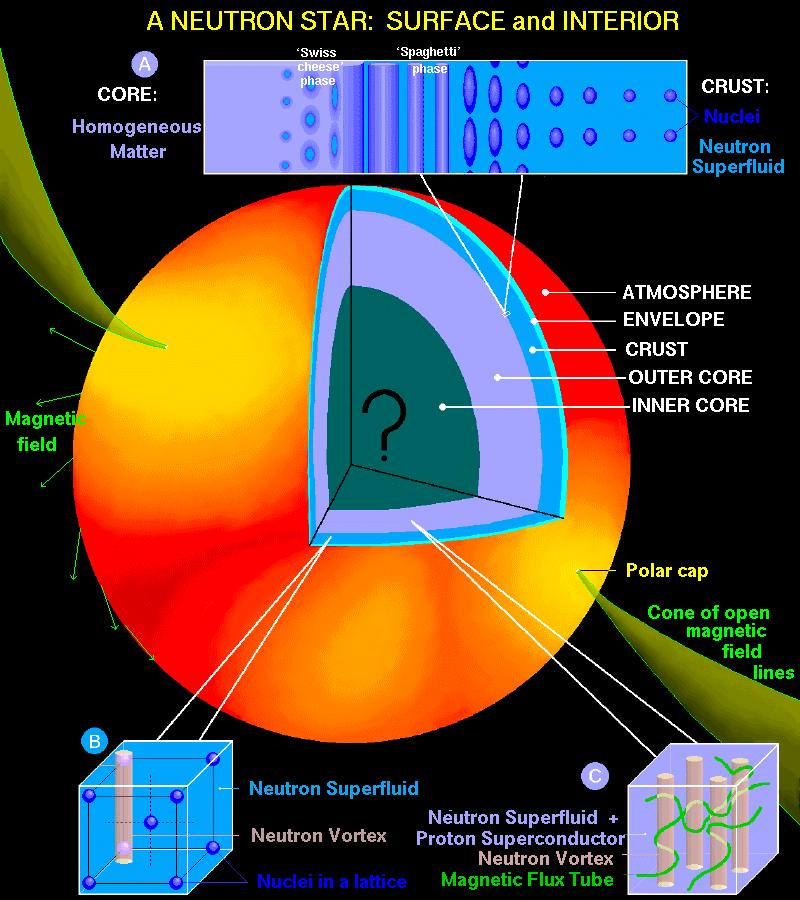
\includegraphics[width=0.8\linewidth]{figures/NStarInt.jpeg}
\end{center}
\caption[Schematic representation of the inside of a neutron star]{Schematic
representation of the inside of an NS. Figure taken 
from~\cite{Page2006}.}\label{fig:NStarInt}
\end{figure}
% 
% description of the structure
The star cools down by emitting photons and neutrinos, and at approximately
$10^8$~K matter is catalyzed, that is in its ground state.
A schematic representation of the internal structure of a cold NS is given in
Fig.~\ref{fig:NStarInt}.
% atmosphere
The outermost surface of an NS consists of a very thin atmosphere of 
only a few centimeters and an envelope of few meters, where the spectrum of
thermal electromagnetic radiation is formed. \edit{The analysis of the thermal 
  emission from the surface layers of isolated NS can provide useful 
  information on the surface temperatures, and the detection of graviationally 
  redshifted spectral lines can yield the NS mass-to-radius ratios.
  Unfortunately, the nonthermal component dominates in the majority of very 
  young pulsars, and for NS older than $\tau \sim 1$ Myr the surface 
  temperature is generally too low to detect the thermal radiation. The thermal 
  radiation from the entire NS surface can dominate at soft x-ray energies for 
  middle-aged pulsars, $\tau \sim 10 - 100$ kyr~\cite{Haensel2007}.} 
% crust
The inhomogeneous crust is situated just below the outermost surface and is 
about $1$~km thick. 
The crust is generally subdivided into two regions: the outer crust and the 
inner crust, and the border between them is situated at the neutron drip 
surface, a few hundred meters from the atmosphere bottom.
Inside the crust, atoms are fully ionized and form a lattice immersed in a
relativistic electron gas, and if the neutron chemical potential is larger than 
the neutron rest mass, additionally in a neutron gas. 
Due to electron capture, matter is more neutron-rich with increasing density, 
further toward the interior of the star.
In the bottom layers of the inner crust, nuclei are expected to exhibit 
nonspherical shapes.
\edit{As the temperature of the inner crust falls below the critical
temperature $T_c \sim 10^{10}$~K, free neutrons with anti-aligned spins and
zero orbital angular momentum form Cooper
pairs and behave in a superfluid state, characterized by the absence of 
viscosity.} 
% core
At about half the saturation density $n_{sat}$, corresponding to the 
equilibrium density of symmetric homogeneous nuclear matter, the crust-core
interface is reached and nuclei disappear. Once again, we can distinguish the
outer core, corresponding to the density range $0.5n_{sat} \lesssim n_B 
\lesssim 2n_{sat}$, and the inner core, where $n_B \gtrsim 2n_{sat}$ ($n_B$
being the baryon density). 
In the outer core, matter consists of a mixture of neutrons, protons, 
electrons, and possibly muons. The composition of the inner core is however 
uncertain, and several hypotheses have been put forward, such as the appearance 
of hyperons, boson condensates, and/or a phase transition to quark 
matter.

\subsection*{Observables of (proto)neutron stars}

Pulsars were identified to rotating NS which produce pulsed emission, soon 
after their chance discovery in 1967 by Jocelyn Bell~\cite{Hewish1968}. Five
decades later, we have now observed about \edit{3000} of them, and numerous 
techniques have been developed to measure their characteristic observables. 

\subsubsection*{Global properties}

% masses
\begin{figure}[!t]
\begin{center}
  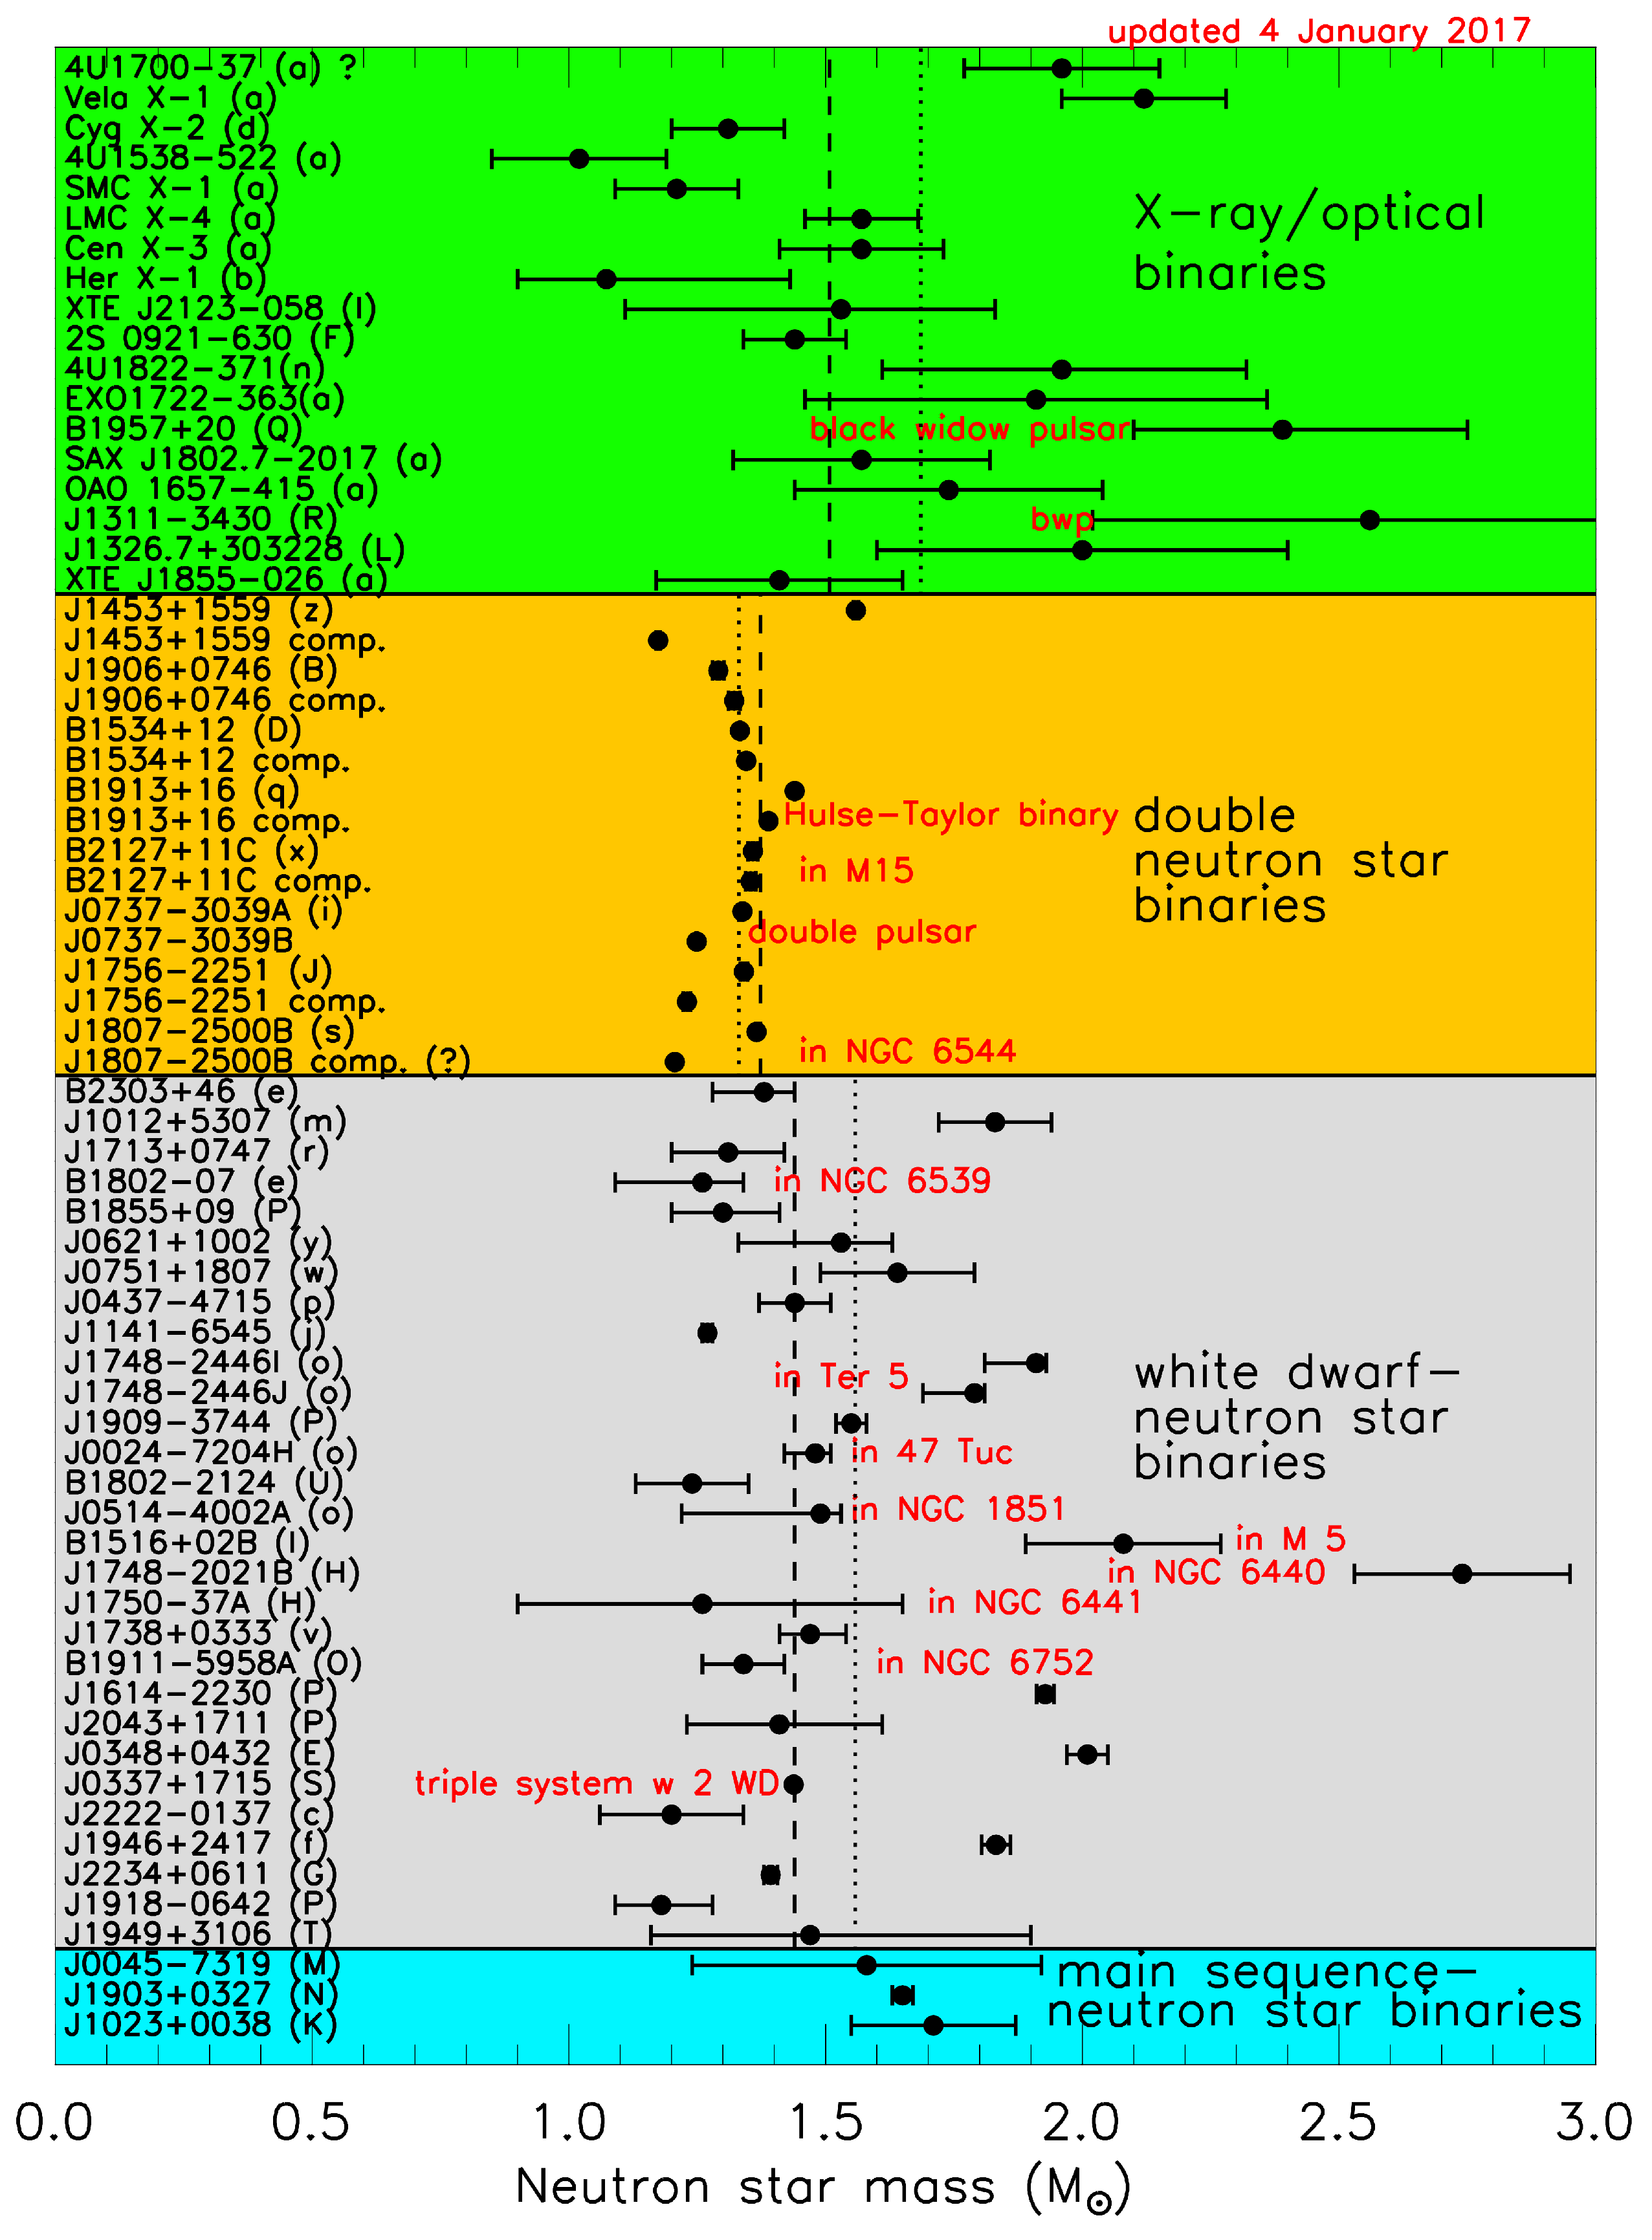
\includegraphics[width=0.7\linewidth]{figures/masses.png}
\end{center}
\caption[Masses measured from pulsar timing]{Masses 
measured from pulsar timing. Vertical dashed (dotted) lines indicate category 
error-weighted (unweighted) averages. Figure taken 
from~\cite{Lattimer2019}.}\label{fig:masses_lattimer}
\end{figure}
%
It is easier for astronomers to measure the mass of an NS belonging to a binary 
system. There are several types of binaries: x-ray binaries, double NS 
binaries, radio pulsar--white dwarf binaries, and \edit{pulsars in binaries 
with nondegenerate stars (main-sequence stars).} Depending on the type 
  of binary, different techniques are used to infer the NS 
  mass~\cite{Haensel2007}.
% Shapiro delay effect - MSP
For example, \edit{in double NS binaries} the relativistic Shapiro 
delay~\cite{Shapiro1964} can be exploited to infer the mass via pulsar timing, 
which consists in the regular monitoring of 
the rotation of a pulsar \edit{over long time periods}. The relativistic 
Shapiro delay is a phenomenon from which precise masses for both a millisecond 
pulsar and its companion can be inferred~\cite{Demorest2010,Cromartie2020}. Let 
us notice however that it is only observed in a small subset of high-precision, 
highly inclined binary pulsar systems. Measured NS masses via pulsar timing are
displayed in Fig.~\ref{fig:masses_lattimer}. 

% Measuring NS radii is less straightforward
Measuring NS radii with high precision is a more challenging task.
The basic principle of the radius extraction relies in the measurement of the 
the x-ray spectrum (flux and frequency), from which both the surface 
temperature and the star radius can be extracted using the equation of 
black-body emission.
In particular, accurate estimations of the star radius are believed to be 
provided by spectral fits in low-mass x-ray binaries (LMXBs) during periods of 
little to no accretion, called quiescence~\cite{Brown1998}.
%
A number of quiescent LMXBs have been studied with the Chandra and/or 
XMM–Newton 
observatories \cite{Heinke2014,Servillat2012,Guillot2014,Guillot2013}.
%
However, the results strongly depend on the assumptions made on the composition
of the neutron star atmosphere which is poorly known~\cite{Steiner2018}. 
An important improvement is expected from the analysis of the recent NICER 
mission, whose first results start to be available 
\cite{Bogdanov2019a,Bogdanov2019b,Miller2019,Raaijmakers2019,Riley2019}, 
even if complications in the interpretation of the 
data arise due to the nonuniformity of the temperature over the surface (hot
spots) \cite{Bogdanov2019a,Bogdanov2019b,Miller2019,Raaijmakers2019,Riley2019}. 
\edit{Typical values} for the NS masses and radii are $M = 1.4M_\odot$ and
$R=10-14$~km, respectively.
 
% tidal
Very recently, the first detection of gravitational waves (GW) from the 
coalescence 
of two NS, the GW170817 event, has yielded important constraints for the tidal 
deformability of NS~\cite{GW1}.
The tidal deformability describes how much a body is deformed by tidal forces,
which arise when two massive bodies are in orbit around each other. 
The simplest and best known example corresponds to the Moon causing the tides 
observed in Earth's oceans.
The detection of gravitational radiation emitted by inspiraling binary NS 
is possible using ground-based GW detectors such as LIGO 
and Virgo. 
Shortly before merging, once the relative distance between the stars is small
enough, the tidal distortion of the NS become so large that, in some cases (in
strongest signals corresponding to closest merging events), it becomes possible 
to infer the tidal deformability from the GW signal. 

\subsubsection*{Pulsar glitches}

% glitches
The so-called pulsar glitches are sudden jumps in the rotational frequency of 
a compact star. They are thought to originate from an abrupt transfer of 
angular momentum from the superfluid components of the NS, acting as an angular 
momentum reservoir, to the solid crust of the star, and all the normal fluid
components which are strongly coupled to the crust by mutual dissipation. This
sudden transfer is thought to be due to the unpinning of the superfluid 
vortices from the crystal lattice~\cite{Anderson1975}. 
%
Indeed, a rotating superfluid, such as the superfluid neutrons in the inner 
crust of the NS, produces individual quantized vortices, with a density 
proportional to the rotational rate. Those vortices migrate towards the surface 
of the star due to the centrifugal force associated to the star rotation, where 
they get pinned to the ions of the lattice that constitutes the solid 
crust of the NS. Since the star experiences a spin-down due to the emission of 
electromagnetic radiation, a differential lag develops between the faster 
superfluid vortices and the slower crust, leading to crustal stress. 
%
When the differential lag between the slower solid crust and faster superfluid 
vortices reach some threshold and can no longer be sustained, the vortices
suddenly unpin from the lattice sites, leading to an angular momentum transfer
to the crust, and the rest of the star which is entangled with the crust by
mutual friction, so as to recover a close equilibrium between the normal and
superfluid components. Since the electromagnetic slowing down is a continuous
process, this is not a final equilibrium situation, and eventually stresses 
start to build up again, ultimately leading to another glitch event.
%
At the time of writing, 555 glitches have been observed in 190 pulsars through 
high-precision pulsar timing~\cite{Espinoza2011,Glitches}. The Vela pulsar 
(PSR B0833-45) is one of the most active glitchers known, with glitches 
occurring four times per decade on average.

\subsubsection*{Cooling of the crust}

\edit{
  Core becomes transparent to neutrinos. However, the presence of impurities in 
  the crust alter transport properties.
  How to measure cooling observables?
}

\section*{Microphysics of the (proto)neutron star crust}

A theoretical description of the different phenomena mentioned above requires 
the modeling of dense baryonic matter, specifically the nuclear equation of 
state (EoS). 
%
The EoS relates, in given conditions of temperature and 
densities, \edit{the thermodynamic quantities of the system, such as the mass
  density and the pressure, at the equilibrium. Its determination allows us 
  to compute} among others the mass-radius relation of NS, obtained by solving 
  the hydrostatic equilibrium equation in general 
  relativity~\cite{Tolman1939,Oppenheimer1939}.
%
Since quantum chromodynamics (QCD) in the nonperturbative regime cannot be 
exactly solved, the EoS is strongly model dependent, which induces considerable 
uncertainties in the prediction of astrophysical observables. 
In this thesis, we are particularly interested in the modeling of the (P)NS 
crust, where matter is inhomogeneous. From the modeling point of view, the 
regime of subsaturation matter is probably the most difficult part of the 
nuclear EoS. Indeed, the uncertainties do not only concern the nuclear energy 
functional, but also the many-body method used to model inhomogeneous matter. 
%
Indeed, the evaluation of the EoS implies to know the microscopic composition 
at each point in the star. At finite temperature, an extra complication arises
from the statistical mechanics treatment of the problem. 
Historically, the stellar EoS at subsaturation 
densities was first calculated within the so-called single-nucleus 
approximation (SNA)~\cite{BBP,Negele1973}, based on the assumption that matter 
can be represented by the most probable nucleus given by the minimization of 
the free energy density of matter. While this approximation is exact at zero
temperature, a full distribution of clusters should be considered at finite
temperature, as is it the case in nuclear statistical equilibrium (NSE) models. 
Again, the exact solution of the many-body problem at finite temperature being 
out of scope, modeling cannot be avoided, which induces a model dependence on 
the calculation of observables. 

One could naively consider that an optimal nuclear model can be extracted by 
confronting the theoretical predictions with the observational data. However, 
a major issue when considering characteristic EoS is that some
observables are better reproduced by a particular model (or a class of 
models), while they fail to reproduce other observables. In addition, each
observable is associated with uncertainties and the ability to reproduce or not 
a determined measurement does not have the same impact on the reliability of
the model, depending on which observable is considered.
In addition to astrophysical constraints, there are also constraints coming
from nuclear experiments, and recent developments in \textit{ab initio} 
calculations based on chiral effective field theory (EFT)~\cite{Drischler2016}, 
which consists in the determination of the nuclear energy functional from a
systematic power expansion which respects the fundamental symmetries of
low-energy QCD~\cite{Machleidt2011}, that is the theory of strong interactions. 
The different models that can be considered have not been confronted to all 
those constraints, and not on the same level. In these circumstances, it is 
very arduous to validate (or invalidate) a model. A solution for this impasse 
is provided by the use of Bayesian inference principle, which allows to update 
our prior beliefs on the EoS with the constraints arising from the multiple 
sources mentioned above.
%
It has been shown that the (P)NS observables are sensitive to the 
microphysics entering the EoS, for instance to the high-order derivatives of 
the nuclear symmetry energy and to the surface properties of finite nuclei. 
It is therefore essential to constrain these inputs in order to control the 
uncertainties in the observables.
In this thesis, we are interested in making realistic predictions and to
investigate the sources of uncertainties in the observables of nonaccreting
cold NS and warm PNS, using the present day constraints provided by nuclear
experiments, theoretical developments in chiral EFT, and astrophysical 
observations. This general argument applies to the total modeling of the 
NS, and also to the NS crust, which is the main focus of this work. 

% niche crust
While the crust only represents a very small percentage of the total NS mass, 
knowledge of it is important in order to understand NS dynamics, notably 
glitches and cooling. In addition to the nuclear EoS, the determination of
crustal observables requires the knowledge of the density and pressure at the
transition point from the solid crust to the liquid 
core~\cite{Piekarewicz2014}.
% glitches: is the crust enough
In order to validate the full crustal origin of the large glitches observed in 
some pulsars, such as Vela, the neutron star crust must be sufficiently thick 
to store a significant amount of angular momentum. The corresponding fraction 
of the crust moment of inertia can be 
estimated~\cite{Link1999,Andersson2012,Delsate2016} in a range going from 
$1.6\%$ up to $15\%$, depending on the importance of the effect of crustal 
entrainment, which is currently under debate~\cite{Martin2016,Watanabe2017}. A 
reliable estimation of the crust thickness and of the associated moment of 
inertia is thus crucially needed to validate the crustal origin of 
pulsar glitches.
%
For all these applications, it is essential to have objective criteria allowing 
to validate or invalidate the different models, and possibly correlate the 
residual uncertainty of model predictions to well-defined parameters that can 
be constrained in the future by more precise experiments or \textit{ab initio} 
calculations. The first part of the present thesis is aimed at providing a step 
forward in this direction. This will be done by introducing a flexible 
metamodeling procedure which will allow us to confront a very large set of 
models of catalyzed nuclear matter to the different constraints coming from 
both low-energy nuclear physics and astrophysical observations of mature 
NS. 

% crystallization
The second part of the thesis will deal with the modeling of the crust at 
finite temperature. Again, the focus will be put on the determination of 
reliable error bars on the determination of astrophysical quantities due to the 
uncertainties of the modeling. This finite temperature modeling is not only 
essential to describe \edit{PNS dynamics}, but it might also be 
relevant for the description of crustal observables of mature neutron stars. 
Indeed, the crust of an NS is unlikely to be in full thermodynamic equilibrium 
at zero temperature: NS are born hot, and if their core cools 
down sufficiently rapidly, the composition might be frozen at a finite 
temperature~\cite{Goriely2011}. 
Deviations from the ground-state composition in the cooled crust around the 
neutron-drip density were already considered in~\cite{Bisnovaty1979}, but 
simple extrapolations of semiempirical mass formulae were used at that time. 
The value of the freeze-out temperature is difficult to evaluate, but a lower 
limit is given by the crystallization temperature, since we can expect that 
nuclear reactions will be fully inhibited in a Coulomb crystal. 
For these reasons, the last part of this thesis will be dedicated to the study 
of the structure of the crust at the temperature of crystallization. 
The possible presence of amorphous and heterogeneous phases in the inner crust 
of a neutron star is expected to reduce the electrical conductivity of the 
crust, with potentially important consequences on the magneto-thermal evolution 
of the star. \edit{The study of cooling processes is important for comparing 
  the theoretical calculations with surface temperature as measured by 
satellites.} In cooling simulations, the disorder is quantified by an impurity 
parameter which is often taken as a free parameter. \edit{This parameter is 
  directly related to the electron--impurity conductivity, which contributes to 
the total thermal conductivity~\cite{Flowers1976}.}

\section*{Structure of the thesis}

% plan
The thesis is divided into three chapters. 
% chapter 1
In Chapter 1, we consider a unified
metamodeling approach in order to calculate the composition and EoS of cold non
accreting NS for any functional of nuclear matter (NM). The cluster energy in
the inner crust is calculated within the compressible liquid drop (CLD)
approximation. 
% chapter 2
In Chapter 2, we carry out the Bayesian determination of the EoS 
parameters, leading to realistic predictions for the observables of cold NS,
which we compare to the constraints of the LIGO/Virgo collaborations.
Valuable information arising from nuclear physics experiments, chiral EFT 
calculations, and astrophysical observations are incorporated into the 
likelihood probability. Correlations among EoS parameters are 
explored. The crust-core transition quantities and fraction of crustal moment
of inertia are computed for the posterior distribution of EoS parameters, and 
we discuss the full crustal origin of Vela pulsar glitches.
% chapter 3
In Chapter 3, we consider an NSE approach to model the crust of PNS at 
finite temperature. The equilibrium composition at the crystallization 
temperature is calculated, and the so-called impurity parameter, which is an 
important input for NS cooling simulations is evaluated for different realistic 
functionals. The presence of odd-mass and odd-charge nuclei in the outer crust
is also investigated.

\clearpage\thispagestyle{empty}
